%TODO: CORREGIR COMANDOS PARA QUE SE VEAN CON VERB
%TODO: INTENTAR QUITAR LA MORRAYA QUE NO SIRVA
%TODO: INTENTAR NO REPETIR TANTAS COSAS EN EL EJERCICIO 3
%TODO: REVISAR DOCUMENTO PARA FALLOS ORTOGRAFICOS/GRAMATICALES
\documentclass{article}
\usepackage[utf8]{inputenc}
\usepackage[spanish]{babel}
\usepackage{graphicx, graphics, float, hyperref}
\usepackage{listings, subcaption}
\usepackage[a4paper, total={6in, 10in}]{geometry}

\title{SSO Práctica 2 Sesión 1}
\author{Andrés Merlo Trujillo}
\date{}
\hypersetup{
    colorlinks=true,
    linkcolor=black,
}

\begin{document}

\maketitle

\tableofcontents

\newpage
%\addcontentsline{toc}{section}{Ejercicio 1}
%\section*{Ejercicio 1}
%\begin{figure}[H]
%    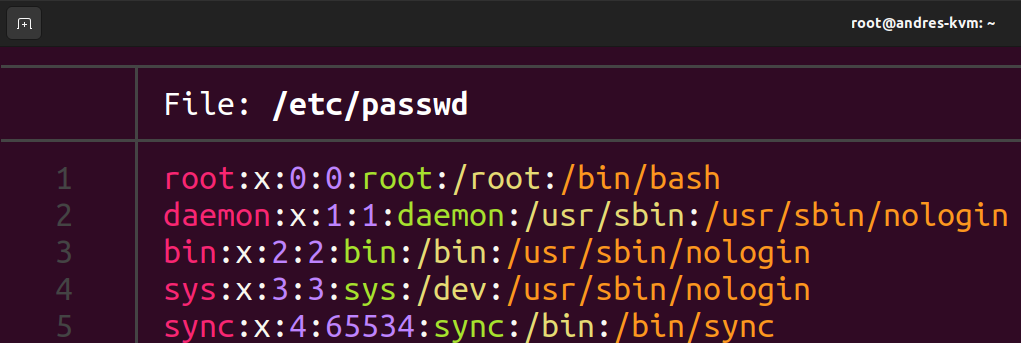
\includegraphics[width=\textwidth]{imagenes/passwdfile.png}
%    \caption{Ejemplo de entradas en el archivo.}
%\end{figure}

\addcontentsline{toc}{section}{Ejercicio 1}
\section*{Ejercicio 1}

Para obtener la arquitectura de la CPU, voy a utilizar la orden \verb|lscpu|.

%foto de lscpu
%Captura desde 2022-11-23 10-33-11


Para saber la distribución, hay dos formas: la primera depende del entorno de escritorios (DE), pero como en mi caso es GNOME 42 se pude hacer yendo a Configuración y Acerca de:

%foto de esta pantalla
%Captura desde 2022-11-23 10-37-46

La segunda opcion es usando el comando \verb|lsb_release -a|, que indica por terminal la misma informacion:

%foto de la salida del comando
%Captura desde 2022-11-23 10-38-58

Ahora, para obtener la version del compilador, se utiliza el comando \verb|gcc --version|:

%foto de la version de gcc
%Captura desde 2022-11-23 10-39-52

Ahora bien, los mecanismos para proteger los binarios ELF son diversos y se encuentran implementados en el kernel y en el compilador. Las protecciones a nivel de kernel son als siguientes:

\begin{itemize}
    \item \textbf{ASLR} (Aleatorizacion de la disposicion del espacio de direcciones): Tiene como objetivo evitar la ejecucion de codigo malicioso como puede ser \textit{shellcode} debido a una funcion del programa vulnerable. ASLR permite aleatorizar en cada ejecucion del programa las distintas partes del mismo, como el codigo del programa, bibliotecas, etc. Esto hace que sea mas dificil que un atacante sepa donde se encuentra la parte vulnerable al ser en cada ejecucion distinta.
\end{itemize}

Mientras que para la parte del compilador hay los siguientes mecanismos:

\begin{itemize}
    \item Proteccion de pila ejecutable
    \item Proteccion de rotura de pila: Mediante el uso de la macro \verb|FORTIFY_SOURCE|, el compilador dará warnings en las secciones de codigo que potencialmente puedan producir un buffer overflow. Además, en tiempo de ejecucion si detecta un buffer oberflow aborta el programa y muestra un log con toda la informacion en el momento del fallo.
    \item Ejecutables independientes de la posicion (PIE): Mediante la opcion del compilador \verb|-pie| se produce un ejecutable independiente de la posicion, esto quiere decir que las distintas partes del programa van a tener un offset para que no se encuentren siempre en una direccion fija.
    \item Fuente fortificada
    \item Protector de pila: Mediante la opcion del compilador \verb|-fstack-protector| que habilita la proteccion de la pila. Hace uso de la tecnica ``Stack Canary'', que es un valor que se le asigna a cada funcion al principio y que al final de la misma se espera que sea igual, si se ha producido un bug o un ataque el programa aborta al ser el valor distinto.
\end{itemize}

\addcontentsline{toc}{section}{Ejercicio 2}
\section*{Ejercicio 2}

\addcontentsline{toc}{subsection}{Apartado A}
\subsection*{Apartado A}

Para que el virus funcione, es necesario modificar el archivo \textit{elfvirus.c} y modificar las llamadas a la funcion \verb|searchForELF| para que use la ruta que he especificado.

%foto de eso
%Captura desde 2022-11-25 17-29-47

A continuacion, es necesario compialr el programa y con la orden \verb|ls -l| se obtiene el tamaño del virus:

%foto del comando
%Captura desde 2022-11-23 12-28-06
%caption: el ejecutbale se llama virus, y como se puede ver tiene un tamaño de 21932

Por tanto, en el define \verb|VIRUS_SIZE| se pone ese tamaño:

%foto del cambio
%Captura desde 2022-11-23 12-29-27

Se compila y ahora al ejecutar el virus infectado aparece lo siguiente:

%foto de la salida del virus
%Captura desde 2022-11-23 12-32-53

Como se puede ver ha infectado el programa \textit{victima}, que es un simple Hola Mundo escrito en C.

Y si ahora ejecuto \textit{victima}, aparece lo siguiente:

%foto de la ejecucion de victima
%victimaInfectada/Captura desde 2022-11-23 12-33-29.png
%aption: se ve que primero se ejecuta el vitus y despues el ejecutable original

Como se puede observar, este programa esta infectado, y si lo pusieramos en otro directorio infectaria a los otros. No obstante, esto no es posible porque en la funcion \verb|searchForELF| se le ha restringido el acceso a solo la carpeta del virus, pero puede tener el potencial de hacer daño.



El script del limpiador tenia ciertos fallos que el interprete detectaba, haciendo que no funcionase. LO he arreglado haciendo las siguientes modificaciones: 

%foto del script limpiador
%caption: se puede ver que ahora uso bash, he cambiado el tamaño del virus, he eliminado el let de ORIG_SIZE y he hecho que ahga bien la cuenta esta misma variable

Despues de estos arreglos, al ejectuarlo aparece l os siguiente:

%foto de la salida
%Captura desde 2022-11-23 12-44-29

Y ahora al ejecutar el ejecutable ``saneado'', aparece la salida correctamente.

El limpiador se podria mejorar haciendo que en vez de tener que ir ejecutable a ejecutbale uno a uno a mano, se pueda pasar un directorio y de manera recursiva vaya limpiando los ejecutables infectados. Para ello, haria falta que el script hiciese una comprobacion de si existe el virus en el ejecutable, ya que siempre intenta eliminar los primeros 21932 Bytes del programa, que es donde reside el virus.

\addcontentsline{toc}{subsection}{Apartado B}
\subsection*{Apartado B}

Usando un editor de texto avanzado o un IDE como Visual Studio Code, se puede ver que la estructura de datos \verb|Elf32_Ehdr| contiene las siguientes arquitecturas (no son todas) en el archivo \verb|elf.h|:

%foto de las arquitecturas
%caption: ALguna de las arquitecturas disponibles
%Captura desde 2022-11-23 13-07-09

Y la lista continua hacia abajo, por lo que solo voy a realizar la comprobacion de si es x86, x86\_64, ARM, ARM64, PowerPC y IA64 (Itanium). Para realizarlo, es necesario usar macros que el compilador \verb|gcc| posee, la lista se encuentra en: \url{https://sourceforge.net/p/predef/wiki/Architectures/}.

Por tanto, el codigo del virus quedaria asi:

%foto del trozo de codigo modificado
%Captura desde 2022-11-25 17-21-11



\end{document}
